\begin{figure}[tb]
    \centering
     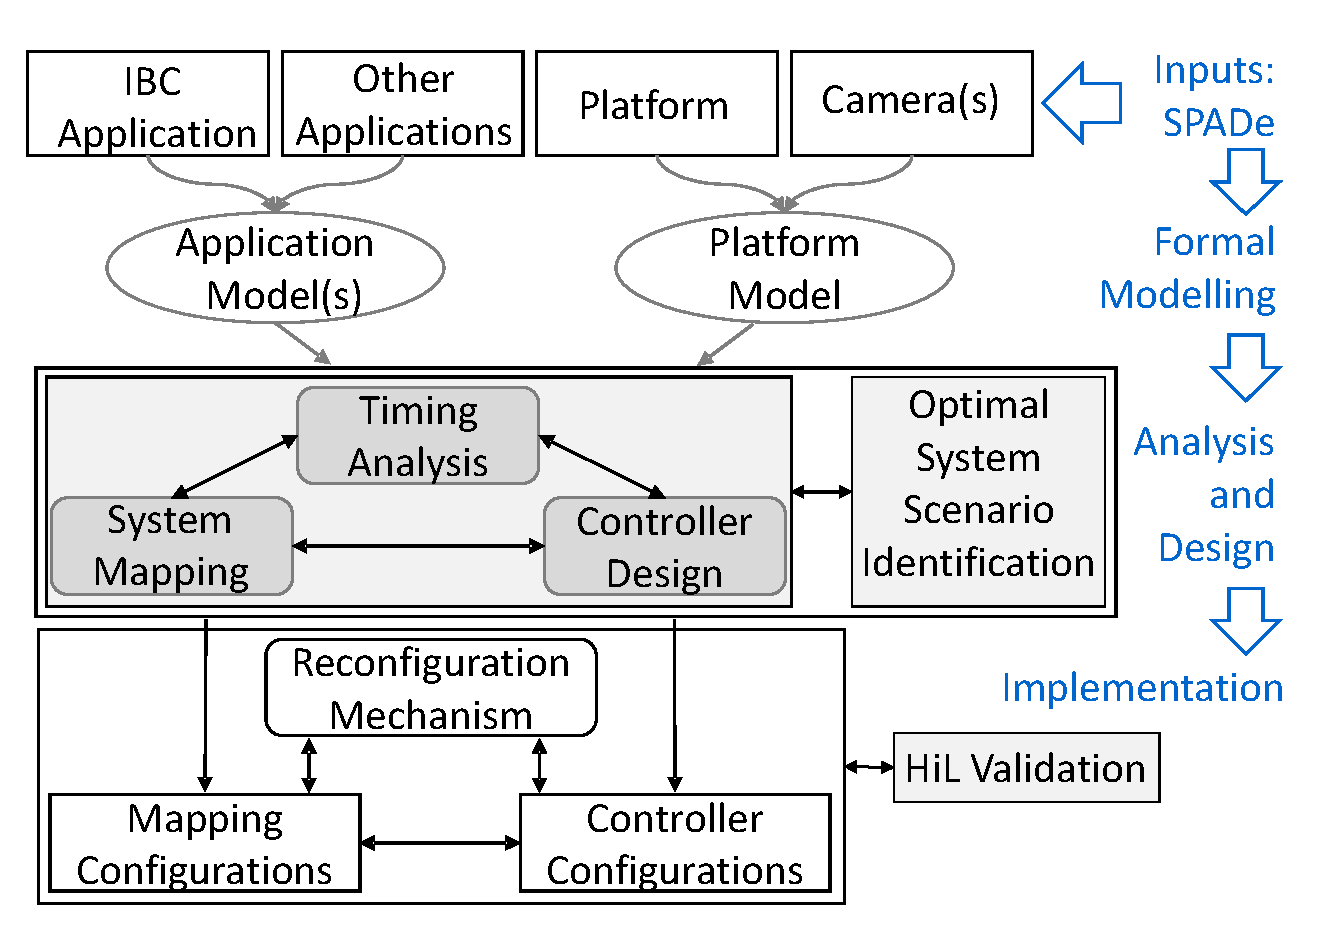
\includegraphics[scale=0.45]{images/SPADe.eps}
    %\vspace{-2em}
    \caption{Overview of the steps in the basic version of the \gls{spade} flow for parallel implementation (adapted from Fig.\ \ref{fig:ch1_spade_overview}, for readability). In a parallel non-pipelined implementation, the sampling period is not constant and can vary at runtime, as opposed to the proposed \gls{spade} flow for pipelined parallelism outlined in Fig.\ \ref{fig:ch1_spade_overview}.}
    \label{fig:ch5_SPADeOverview}
\end{figure}

The basic \gls{spade} flow comprises the following steps as shown in Fig.~\ref{fig:ch5_SPADeOverview} (adapted from Fig.\ref{fig:ch1_spade_overview}): 
\begin{enumerate}
    \item identify, model and characterise the frequently occurring workload scenarios that characterise the dynamic behaviour of the image processing in the control loop;
    
    \item find optimal mappings for these scenarios for the given platform allocation;
    
    \item identify optimal system scenarios combining workload and mapping information and taking into account constraints from the control domain, e.g. stability, and from the embedded domain, e.g. camera frame rate; 
    
    \item design a controller with high overall \gls{qoc} and guaranteed stability for the chosen system scenarios; and

    \item a runtime reconfiguration mechanism for implementation.
\end{enumerate}
As already stated, we illustrate the \gls{spade} flow considering the predictability and composibility properties of the \gls{compsoc} platform. In the following, we detail the steps in the \gls{spade} flow.